% This is "sig-alternate.tex" V1.9 April 2009
% This file should be compiled with V2.4 of "sig-alternate.cls" April 2009
%
% This example file demonstrates the use of the 'sig-alternate.cls'
% V2.4 LaTeX2e document class file. It is for those submitting
% articles to ACM Conference Proceedings WHO DO NOT WISH TO
% STRICTLY ADHERE TO THE SIGS (PUBS-BOARD-ENDORSED) STYLE.
% The 'sig-alternate.cls' file will produce a similar-looking,
% albeit, 'tighter' paper resulting in, invariably, fewer pages.
%
% ----------------------------------------------------------------------------------------------------------------
% This .tex file (and associated .cls V2.4) produces:
%       1) The Permission Statement
%       2) The Conference (location) Info information
%       3) The Copyright Line with ACM data
%       4) NO page numbers
%
% as against the acm_proc_article-sp.cls file which
% DOES NOT produce 1) thru' 3) above.
%
% Using 'sig-alternate.cls' you have control, however, from within
% the source .tex file, over both the CopyrightYear
% (defaulted to 200X) and the ACM Copyright Data
% (defaulted to X-XXXXX-XX-X/XX/XX).
% e.g.
% \CopyrightYear{2007} will cause 2007 to appear in the copyright line.
% \crdata{0-12345-67-8/90/12} will cause 0-12345-67-8/90/12 to appear in the copyright line.
%
% ---------------------------------------------------------------------------------------------------------------
% This .tex source is an example which *does* use
% the .bib file (from which the .bbl file % is produced).
% REMEMBER HOWEVER: After having produced the .bbl file,
% and prior to final submission, you *NEED* to 'insert'
% your .bbl file into your source .tex file so as to provide
% ONE 'self-contained' source file.
%
% ================= IF YOU HAVE QUESTIONS =======================
% Questions regarding the SIGS styles, SIGS policies and
% procedures, Conferences etc. should be sent to
% Adrienne Griscti (griscti@acm.org)
%
% Technical questions _only_ to
% Gerald Murray (murray@hq.acm.org)
% ===============================================================
%
% For tracking purposes - this is V1.9 - April 2009

\documentclass[A4]{sig-alternate}

\usepackage{nicefrac}
\usepackage{array}
\usepackage[numbers]{natbib}
\usepackage{multirow}
\usepackage{booktabs}

\newcolumntype{C}[1]{>{\centering\arraybackslash\hspace{0pt}}p{#1}}
\newcolumntype{L}[1]{>{\raggedright\arraybackslash\hspace{0pt}}p{#1}}
\newcolumntype{R}[1]{>{\raggedleft\arraybackslash\hspace{0pt}}p{#1}}

\newcommand{\shl}{\,\texttt{<}\texttt{<}\,}
\newcommand{\shr}{\,\texttt{>}\texttt{>}\,}
\newcommand{\sar}{\,\texttt{>}\texttt{>}\texttt{>}\,}


\pagestyle{empty}    %%%%%% <- remove this line to enable page numbering
\begin{document}
\setcounter{page}{1} %%%%%% <- change this number to set the starting page number




% --- Author Metadata here ---
\conferenceinfo{SAICSIT}{'15, September 28-30, Stellenbosch, South Africa}
\CopyrightYear{2015} % Allows default copyright year (200X) to be over-ridden - IF NEED BE.
\crdata{} % Allows default copyright data (0-89791-88-6/97/05) to be over-ridden - IF NEED BE.
% --- End of Author Metadata ---


% --- fix sig-alternate copyright block spacing ---
\makeatletter
\def\@copyrightspace{
\@float{copyrightbox}[b]
\begin{center}
\setlength{\unitlength}{1pc}
\begin{picture}(20,7)         %%%%%% <- This fixes the amount of space reserved for the copyright message
\put(0,-0.95){\crnotice{\@toappear}}
\end{picture}
\end{center}
\end@float}
\makeatother
% --- fix sig-alternate copyright block spacing ---


% --- Altered ACM Metadata here ---
%%%%%%\permission{Permission to make digital or hard copies of all or part of this work for personal or classroom use is granted without fee provided that copies are not made or distributed for profit or commercial advantage and that copies bear this notice and the full citation on the first page. Copyrights for components of this work owned by others than the author(s) must be honored. Abstracting with credit is permitted. To copy otherwise, or republish, to post on servers or to redistribute to lists, requires prior specific permission and/or a fee. Request permissions from Permissions@acm.org.}
%%%%%%
%%%%%%\global\copyrightetc{
%%%%%%Copyright is held by the owner/author(s). Publication rights licensed to ACM.
%%%%%%ACM 978-1-4503-2112-9/13/10...\$15.00.\\
%%%%%%http://dx.doi.org/10.1145/2513456.2513501
%%%%%%}
% --- Altered ACM Metadata here ---




\title{A Register-Mapped Virtual Machine}
%
% You need the command \numberofauthors to handle the 'placement
% and alignment' of the authors beneath the title.
%
% For aesthetic reasons, we recommend 'three authors at a time'
% i.e. three 'name/affiliation blocks' be placed beneath the title.
%
% NOTE: You are NOT restricted in how many 'rows' of
% "name/affiliations" may appear. We just ask that you restrict
% the number of 'columns' to three.
%
% Because of the available 'opening page real-estate'
% we ask you to refrain from putting more than six authors
% (two rows with three columns) beneath the article title.
% More than six makes the first-page appear very cluttered indeed.
%
% Use the \alignauthor commands to handle the names
% and affiliations for an 'aesthetic maximum' of six authors.
% Add names, affiliations, addresses for
% the seventh etc. author(s) as the argument for the
% \additionalauthors command.
% These 'additional authors' will be output/set for you
% without further effort on your part as the last section in
% the body of your article BEFORE References or any Appendices.

\numberofauthors{2} 

\author{
% You can go ahead and credit any number of authors here,
% e.g. one 'row of three' or two rows (consisting of one row of three
% and a second row of one, two or three).
%
% The command \alignauthor (no curly braces needed) should
% precede each author name, affiliation/snail-mail address and
% e-mail address. Additionally, tag each line of
% affiliation/address with \affaddr, and tag the
% e-mail address with \email.
%
% 1st. author
\alignauthor
Matthew Sainsbury\\
       \affaddr{Computing Sciences}\\
       \affaddr{Nelson Mandela Metropolitan University}\\
       \affaddr{Port Elizabeth, South Africa}\\
       \email{matthew@sainsbury.za.net}
\alignauthor
Kevin A. Naud\'{e}\\
       \affaddr{Computing Sciences}\\
       \affaddr{Nelson Mandela Metropolitan University}\\
       \affaddr{Port Elizabeth, South Africa}\\
       \email{Kevin.Naude@nmmu.ac.za}
}
% There's nothing stopping you putting the seventh, eighth, etc.
% author on the opening page (as the 'third row') but we ask,
% for aesthetic reasons that you place these 'additional authors'
% in the \additional authors block, viz.
\date{19 May 2015}
% Just remember to make sure that the TOTAL number of authors
% is the number that will appear on the first page PLUS the
% number that will appear in the \additionalauthors section.

\maketitle
\begin{abstract}
Traditional JIT-less high-level register virtual machines simulate virtual registers in random access memory (RAM) and load virtual registers from RAM whenever they are accessed \citep{caseregistervm}. An alternative approach is investigated where virtual registers are mapped to physical machine registers, and instructions are dispatched not only on the opcode, but also on the operands of the instruction. To emulate a virtual instruction, the interpreter jumps to the appropriate code segment in a table of implementation code based on the instruction word to be executed.
\end{abstract}

% A category with the (minimum) three required fields
\category{C.0}{Computer Systems Organization}{General}

\terms{Virtual Machines, ISA, Interpreters}

\keywords{Instruction Set Architecture, Register Machine}

\section{Introduction}

High level language interpreters are typically implemented with a compiler that compiles the input source code into an intermediary bytecode, which is then interpreted on a high level virtual machine. High level virtual machines are not simply system virtual machines that emulate a real instruction set architecture (ISA) \citep{smithvmarticle}. Instead, they execute bytecode for a machine imagined by the developer which is typically more sophisticated and generic than any real machine's ISA. This ``imaginary'' machine more easily supports the high-level nature of typical interpreted languages and---crucially---is not tied to any specific real architecture. The practice of translating a high level interpreted language into an intermediary bytecode also helps modularize the structure of the interpreter by separating the language and context analysis structures from the host-specific implementation details \citep{structureinterpreters}.

Traditionally, the high level virtual machines implemented in interpreters are stack machines. Instructions for stack machines are smaller, because instruction operands are implicit. This means that instruction fetching is faster. It is easier to compile code for a stack machine than a register machine because the compiler does not need to implement a register allocator \citep{caseregistervm}.

On the other hand, register-based machines have some advantages over stack-based machines. For instance, many tasks can be performed in fewer register instructions than stack instructions \citep{caseregistervm}. Most real machines are register machines, so there is more opportunity for register virtual machines to take advantage of the host machine hardware. \citet{stackregistershowdown} found that an efficient register virtual machine can execute benchmarks 32\% faster than an analogous stack machine.

\section{Just-In-Time Compilation}
Executing bytecode on any virtual machine is significantly slower than executing native code \citep{optimizingindirectbranch}. Just-in-time (JIT) compilation tries to bring ``the best of both worlds'' together. Modern JIT interpreters begin with the normal interpretation process, but while interpreting, profiles the executing bytecode to determine which parts of the bytecode would most benefit from native execution. Once it has identified these sections of bytecode, it compiles them into the host machine's instruction set and executes them natively instead of interpreting them \citep{historyjit}.

\subsection{Problems with JIT}
Although JIT compilation is a good strategy to improve the performance of virtual machines, they have disadvantages in certain use cases---for instance, in multi-instance programs, where many identical threads of the same code are executed simultaneously. A real-world example of such a program is a web server, which spawns several identical program threads to serve web clients asynchronously.

Native multi-instance programs share a read-only code space between instances. This is not possible in JIT interpreters because a JIT compiler alters the program code as it runs. A JIT compiler cannot do this with a shared code space because an in-progress JIT compilation might interfere with a thread executing the same part of the program. The alternative is to maintain a separate code space for each process, which is wasteful because it means that the JIT compiler will compile interpreted code separately for every running instance---essentially translating the same code over and over. It is useful to explore opportunities for improvement in JIT-less interpreters so that situations where JIT compilation is inappropriate are not neglected.



%Because most hosts are register machines, it would seem like a good idea to try to map virtual registers to real host registers. Unfortunately, unlike virtual registers that are implemented in host memory, real registers cannot be accessed by reference \citep{caseregistervm}. This complicates writing host implementations of virtual machine instructions because it means that a different version of implementing code must be written for every combination of virtual machine operands. Despite these difficulties, it is worthwhile to investigate designs of JIT-less register virtual machines that attempt to narrow the divide between the host and the guest architecture.


\section{Project Goals} 
The goal of the project is to investigate the feasibility of register-mapped virtual machines for interpreters running on a modern architecture. To this end, a high-level, register-mapped virtual machine has been designed, and is to be implemented and evaluated.

This virtual machine will have some unique design details that have not before been investigated or thought feasible. It will map some virtual machine registers to real registers. The virtual machine will perform dispatch not only on the opcodes of instructions, but on the entire instruction word including operands. The instruction word will be dispatched to a code table containing a subroutine for every combination of virtual machine opcode and operands. This is necessary because there is no operand fetch mechanism that makes sense for a register-mapped virtual machine. (Where would you store it?)

Such a code table is likely to be very large, since it grows polynomially with the number of opcodes and operands. Because of the adverse possibility of code explosion, the overarching design principle for the architecture was to reduce the number of different opcodes, because each instance of the opcode means a case in the implementation table. This is especially important for instructions that operate over many operands, because each additional operand in an instruction increases the size of the implementation code for the instruction by a factor of the number of registers.

The virtual machine targets the Intel 64 host machine architecture, and is written mostly in assembly, with some operating system-facing code written in C for ease of development. The virtual machine must be written in assembly to obtain the level of system control needed to perform register mapping. To remain practical, a method will be developed to generate implementation code automatically for every combination of virtual opcode and operands.

To aid in evaluation of the design, two other virtual machines will also be developed that support an identical instruction set. One will be a traditional virtual machine. The aim of this machine is to be a baseline comparison for the other machines. For the sake of fair comparison, the traditional machine will be as similar as possible to the register-mapped machine, except in the main detail of interpreting instructions, where the traditional machine will deviate and implement a traditional fetch-decode-execute-store process. This will require a specialized bytecode format, as discussed later. Unlike the register-mapped virtual machine, it will store virtual registers in a location in physical memory. The second alternative virtual machine is a compromise between the traditional virtual machine and the register-mapped machine. This machine will not be register mapped, but retains the large table of specialized implementation code. This virtual machine is useful in determining whether the difficulty of assembly programming is worth mapping registers.

To compare these three machines, several benchmark programs will be used to test the machines. These benchmarks have been chosen to test a realistically wide range of runtime behaviours, such as integer arithmetic, string manipulation and data structure traversal. Each benchmark has been hand-written in the instruction set of the two machines. The results of these benchmarks should provide some meaningful information about the appropriateness of the new design over traditional register virtual machines.


\section{Design}

\subsection{Instruction Set Architecture (ISA)}
The virtual machine designed is statically typed. It has six 64-bit general-purpose registers \texttt{r0} through \texttt{r5}. These are notionally either integers or pointers. Instructions expect certain combinations of integers and pointers, but it is the responsibility of the programmer to ensure that they are given the correct operands, and there is no run-time type checking. Internally, there is also a instruction pointer (\texttt{pc}) and frame base pointer, (\texttt{fbp}) but these are implicit and only feature indirectly in the instruction set.

In many instruction sets, opcode and operands are seperated into bit fields in the instruction word. Such a structure is usually designed so that conventional virtual machines can easily extract the operand portion of the instruction during operand fetching. Only the traditional virtual machine implements instructions this way. The bitfield structure serves no purpose in the register-mapped virtual machine, because instruction dispatch is performed over the entire instruction set. In fact, in the register-mapped virtual machine, opcodes can be entirely arbitrary. However, for ease of code generation, instruction codes are grouped by opcode and follow a regular pattern based on the instruction's operands.

Instruction words are sixteen bits long. Certain instructions are followed by two-byte immediate values. Some immediates serve as signed relative displacement pointers to eight-byte aligned, eight-byte integer constants. Other immediates are signed displacements for jumps, or displacements to functions or data structure prototypes.

The instruction set was designed to be as small as possible. This means that many conventional instructions have been removed because they can be accomplished by another instruction. An example of this is that the instruction set does not contain a \texttt{subc} instruction to subtract an immediate constant from a register. Instead, this is accomplished by the \texttt{addc} instruction with a negative constant. Another application of this design decision is in instructions such as the \texttt{and} and \texttt{or} instruction, where the trivial cases, \texttt{x\,\&\,x} and \texttt{x\,|\,x} are forbidden because they never achieve anything useful.

\subsection{Virtual Machine}

Most efficient interpreters dispatch on instructions as shown in Figure~\ref{code:interpreter}. An instruction is fetched, decoded, and its opcode is isolated. The opcode is used as an index into a jump table, here called \texttt{vector}. A jump is made to specialized code for the opcode to be executed. This code isolates the operand portion of the instruction, and fetches the register values from memory and stored in registers. The actual operation is executed, and the result is moved back into memory. The next instruction is fetched and the process continues. As has been demonstrated, the virtual machine does a lot of work decoding instructions and fetching operands, compared to actually executing the interpreted code. 

\begin{figure}
	\begin{center}
		\begin{minipage}[b]{0.8\linewidth}
			\begin{verbatim}
			vector: ;jump table
			  dq add
			  dq sub
			  ...
			
			add:
			  ;decode add instruction
			  ;fetch register operands from memory
			  mov rbx, [registers+{op1}]
			  mov rcx, [registers+{op2}]
			  add rbx, rcx ;actual operation
			  mov [registers+{op1}], rbx
			  ;fetch and decode next instruction
			  jmp [vector+{opcode}]
			
			sub:
			  ...
			\end{verbatim}
			\caption{Implementation Of A Typical Interpreter}
			\label{code:interpreter}
		\end{minipage}
	\end{center}
\end{figure}

In the register-mapped interpreter, fetching operands and storing results is not needed, because virtual registers remain in physical registers. Additionally, because of the table of implementation code, there is no instruction decode. The implementation of this is shown in Figure~\ref{code:registermapped}. As before, a jump table called \texttt{vector} is used, but it is now significantly larger. the entire instruction word is used as an index over the jump table to jump straight into the implementation code for the instruction. The very first step in this code is to execute the instruction, because there is no operand fetch stage. The next instruction is then fetched through \texttt{lodsw} and the process continues.

\begin{figure}
	\begin{center}
		\begin{minipage}[b]{0.8\linewidth}
			\begin{verbatim}
			vector:
			  dq add_r0_r0
			  dq add_r0_r1
			  ...
			
			add_r0_r0:
			  add rbx, rbx
			  lodsw ;load next instruction
			  jmp [vector+rax*8]
			
			add_r0_r1:
			  add rbx, rcx
			  lodsw
			  jmp [vector+rax*8]
			\end{verbatim}
			\caption{Implementation Of Register-Mapping}
			\label{code:registermapped}
		\end{minipage}
	\end{center}
\end{figure}

In this design, we trade all the intricacies of the decode, fetch, and store steps of normal interpreters for lots of specialized code. Previously, this was not viable because CPUs had very small amounts of instruction cache \cite{stackcaching}. However, modern processors have much larger instruction caches, making this approach more interesting. In fact, we expect the interaction between code size and instruction cache size to be a large factor in the success of this design of virtual machine. 

\subsection{Implementation Code Generation}
Writing hundreds of instances of very similar code by hand is not possible. A Ruby script is used to automate the arduous task of writing this code. Prototypes of implementation code for each opcode were written in a simplified version of the Liquid templating language. Figure~\ref{code:template} shows an example of such a template---here for the \texttt{jeqp} instruction which does a conditional branch based on the equality of two pointers. Text surrounded by \texttt{\{...\}} is tranformed by the templating engine.

For instructions with operands, variables \texttt{i}, \texttt{j} and \texttt{k} hold the index of the register in operand 1, 2, and 3 respectively. This holds similarly for instructions that take only one or two operands. The array \texttt{r} referred to in the template holds the register mapping between virtual and physical machines. Thus \texttt{"\{r[0]\}"} results in an output of \texttt{"rbx"}. Similarly, \texttt{s} is a list of scratch registers available for use.

\begin{figure}
	\begin{center}
		\begin{minipage}[b]{0.8\linewidth}
			\begin{verbatim}
			cmp {r[i]}, {r[j]}
			jne .ne
			movsx {s[0]}, word [rsi]
			jmp .end
			.ne:
			movsx {s[0]}, word [rsi+2]
			.end:
			add rsi, {s[0]}
			\end{verbatim}
		\end{minipage}
		\caption{Sample Implementation Template}
		\label{code:template}
	\end{center}
\end{figure}
Liquid also allows more advanced templating---such as if-statements---for trickier implementations where specific operands need even more specialized code. This need did arise for operations such as div, where the underlying division instruction on Intel 64 requires operands in specific registers.

These templates are instantiated \textit{en masse}, combined with the rest of the code for the virtual machine and assembled. Currently, the code size of the register-mapped virtual machine is about 15 000 lines of assembly. This becomes an executable of about 60KB.

\section{Preliminary Results}
This project is not yet complete. While the virtual machines are almost feature-complete, (lacking a garbage collector at this stage) a lot of work must still be done to profile and analyse the control path in these virtual machines to get them to their optimal, before they can be compared against each other. The benchmarks also have a lot of scope to be optimized.
\begin{figure}
	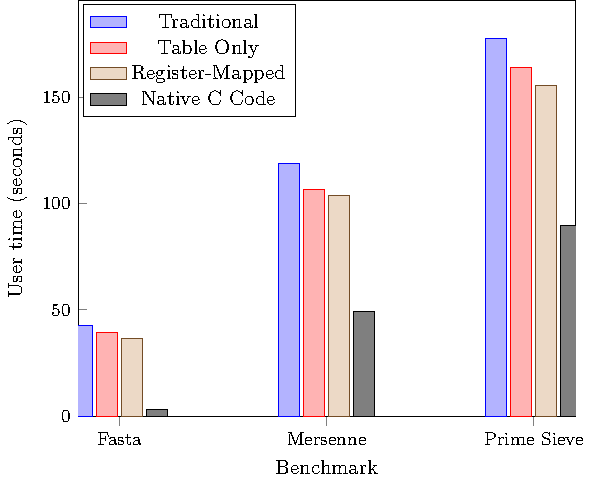
\includegraphics{plot}
	\caption{Initial Benchmark Results}
	\label{fig:bench}
\end{figure}
However, a full run of benchmarks was completed on an Intel Haswell Core i5 processor. Each benchmark was run on each virtual machine ten times and an agreggate time was recorded. These times are recorded in Figure~\ref{fig:bench}.

The register-mapped virtual machine is faster than the traditional virtual machine in all benchmarks. However, there is only about a 12\% increase in speed on average, which is quite disappointing.


\sloppy % latex freaks out without this
The virtual machine that is a compromise between the register-mapped and traditional virtual machine shows promise. It is closer in performance to the register-mapped machine than to the traditional machine. This suggests that the strategy of a large implementation table may be able to be applied to higher level languages such as C. 

\section{Conclusions}
\label{sec:conclusion}
Although JIT has dominated the attention of research effort in the virtual machine interpreter field, there are some applications for which JIT is not an ideal solution. It is therefore important that research is done into alternative approaches that are applicable, especially since the current processor architecture landscape has changed significantly since the majority of research on non-JIT interpreters was done, with the advent of large cache sizes and more complex processors.

Two new approaches to JIT-less interpreters have been presented and tentatively examined. The first is a dispatch over the entire instruction word, and the associated large table of implementation code. First results indicate that this is the more promising of the two approaches, and its applications outside of novelty assembly-based virtual machines remains to be seen.

The other is mapping virtual machine register to the underlying hardware registers. According to initial results, the development pain to accomplish this is not rewarded by a significant increase in virtual machine performance.

It is important to stress that the work previewed in this report is not complete, and further auditing, improvements and analysis are likely to change the tone of this story.


\section{Acknowledgments}
My friend and fellow student Douglas Bentley is a co-author of the virtual machine's instruction set, and was a great help during the implementation and testing of the benchmarks featured in this report.

The financial assistance of the National Research Foundation (NRF) towards this research is hereby acknowledged. Opinions expressed and conclusions arrived at, are those of the author and are not necessarily to be attributed to the NRF.

%
% The following two commands are all you need in the
% initial runs of your .tex file to
% produce the bibliography for the citations in your paper.
\bibliographystyle{abbrvnat}

\bibliography{references}



% You must have a proper ".bib" file
%  and remember to run:
% latex bibtex latex latex
% to resolve all references
%
% ACM needs 'a single self-contained file'!
%
%APPENDICES are optional
\balancecolumns
%\appendix
%Appendix A




%\balancecolumns % GM June 2007
% That's all folks!


\end{document}
